\documentclass[english]{tktltiki}
\usepackage[pdftex]{graphicx}
\usepackage{subfigure}
\usepackage{booktabs}
\usepackage{url}
\usepackage{amsthm,amssymb}
\usepackage{amsmath}
\usepackage{todonotes}

\begin{document}
\onehalfspacing

\title{Interactive Office Project}
\author{Jan Lippert, Luca Vitrini, Michael Morasch, P�ter Ivanics}
\date{\today}

\maketitle

\numberofpagesinformation{\numberofpages\ pages + \numberofappendixpages\ appendices}
\mytableofcontents

\section{Introduction}
% introductory summary to the context

% what is this report about? under what circumstances the project is carried out? 
This report is a summary for the Interactive Office project carried out in the Designing Interactive Systems course at the Department of Computer Science at University of Helsinki during the Spring term of 2017. The report introduces the project ideas, scope, presents its timeline, findings and results.

% what is the goal of this document?
The goal of this document to summarize the utilized methods, identified problems, describe the challenges and findings encountered by the researchers during the project. To make the report easier to read and understand, the chapters to follow are in chronological order similarly to the flow of the project.

\section{Topic selection and research area}
% the context in which the course was started
During the course lectures, several areas of Human-Computer Interaction (HCI) and related areas were presented and discussed. The course material covered several aspects of research in this area, such as user research, needfinding, prototyping methods and product evaluation. Furthermore, popular areas of research, such as augmented and virtual reality, ubiquitous computing, physiological computing were discussed. 

% what were the original ideas and how the interactive office came to surface?
The topic of Smart Home applications was one of the possible research to dive into, which served as the origin of the present research. Despite the fact that the technology in such application field is studied for a long time already, the solutions are yet limited to the home/living environment. By living environment we mean a setting, where people live either on their own or in a family, perform household-related activities (e.g. cooking, cleaning), spend their free time together and so on. At the same time, Smart Home solutions bring running a household to a new level by introducing interactive, computer-facilitated solutions to enhance energy-efficiency and well-being of families. 

% how does our idea differ, what are the main similarities and differences? 
At the first place our group started thinking, how such solutions could be utilized in a different setting, such as an office or a working environment. Starting from existing Smart Home solutions we could derive several aspects that could be brought into a Smart Office solution, such as: 

\begin{itemize}
	\item energy-efficiency, 
	\item automation of recurring tasks,
	\item well-being of employees in the office,
	\item enhancement of work culture and atmosphere, 
	\item workforce management, workload tracking and optimization,
	\item efficient maintenance of electronic devices and facilities.
\end{itemize}

% why is this research area important? 
Undoubtedly, the above aspects are relevant in numerous places and setting. For example, companies that operate in any field of industry are likely to have an office, where the employees do their everyday job. Naturally, it is in the interest of the corporation to address the aspects listed above to enhance efficiency, quality work and atmosphere. 

\section{Needfinding}
\subsection{Stakeholder analysis}
% who are the stakeholders? 

	\todo{We should redraw this in Visio or similar software - Peter}
	\begin{figure}[h] 
		\begin{center}
			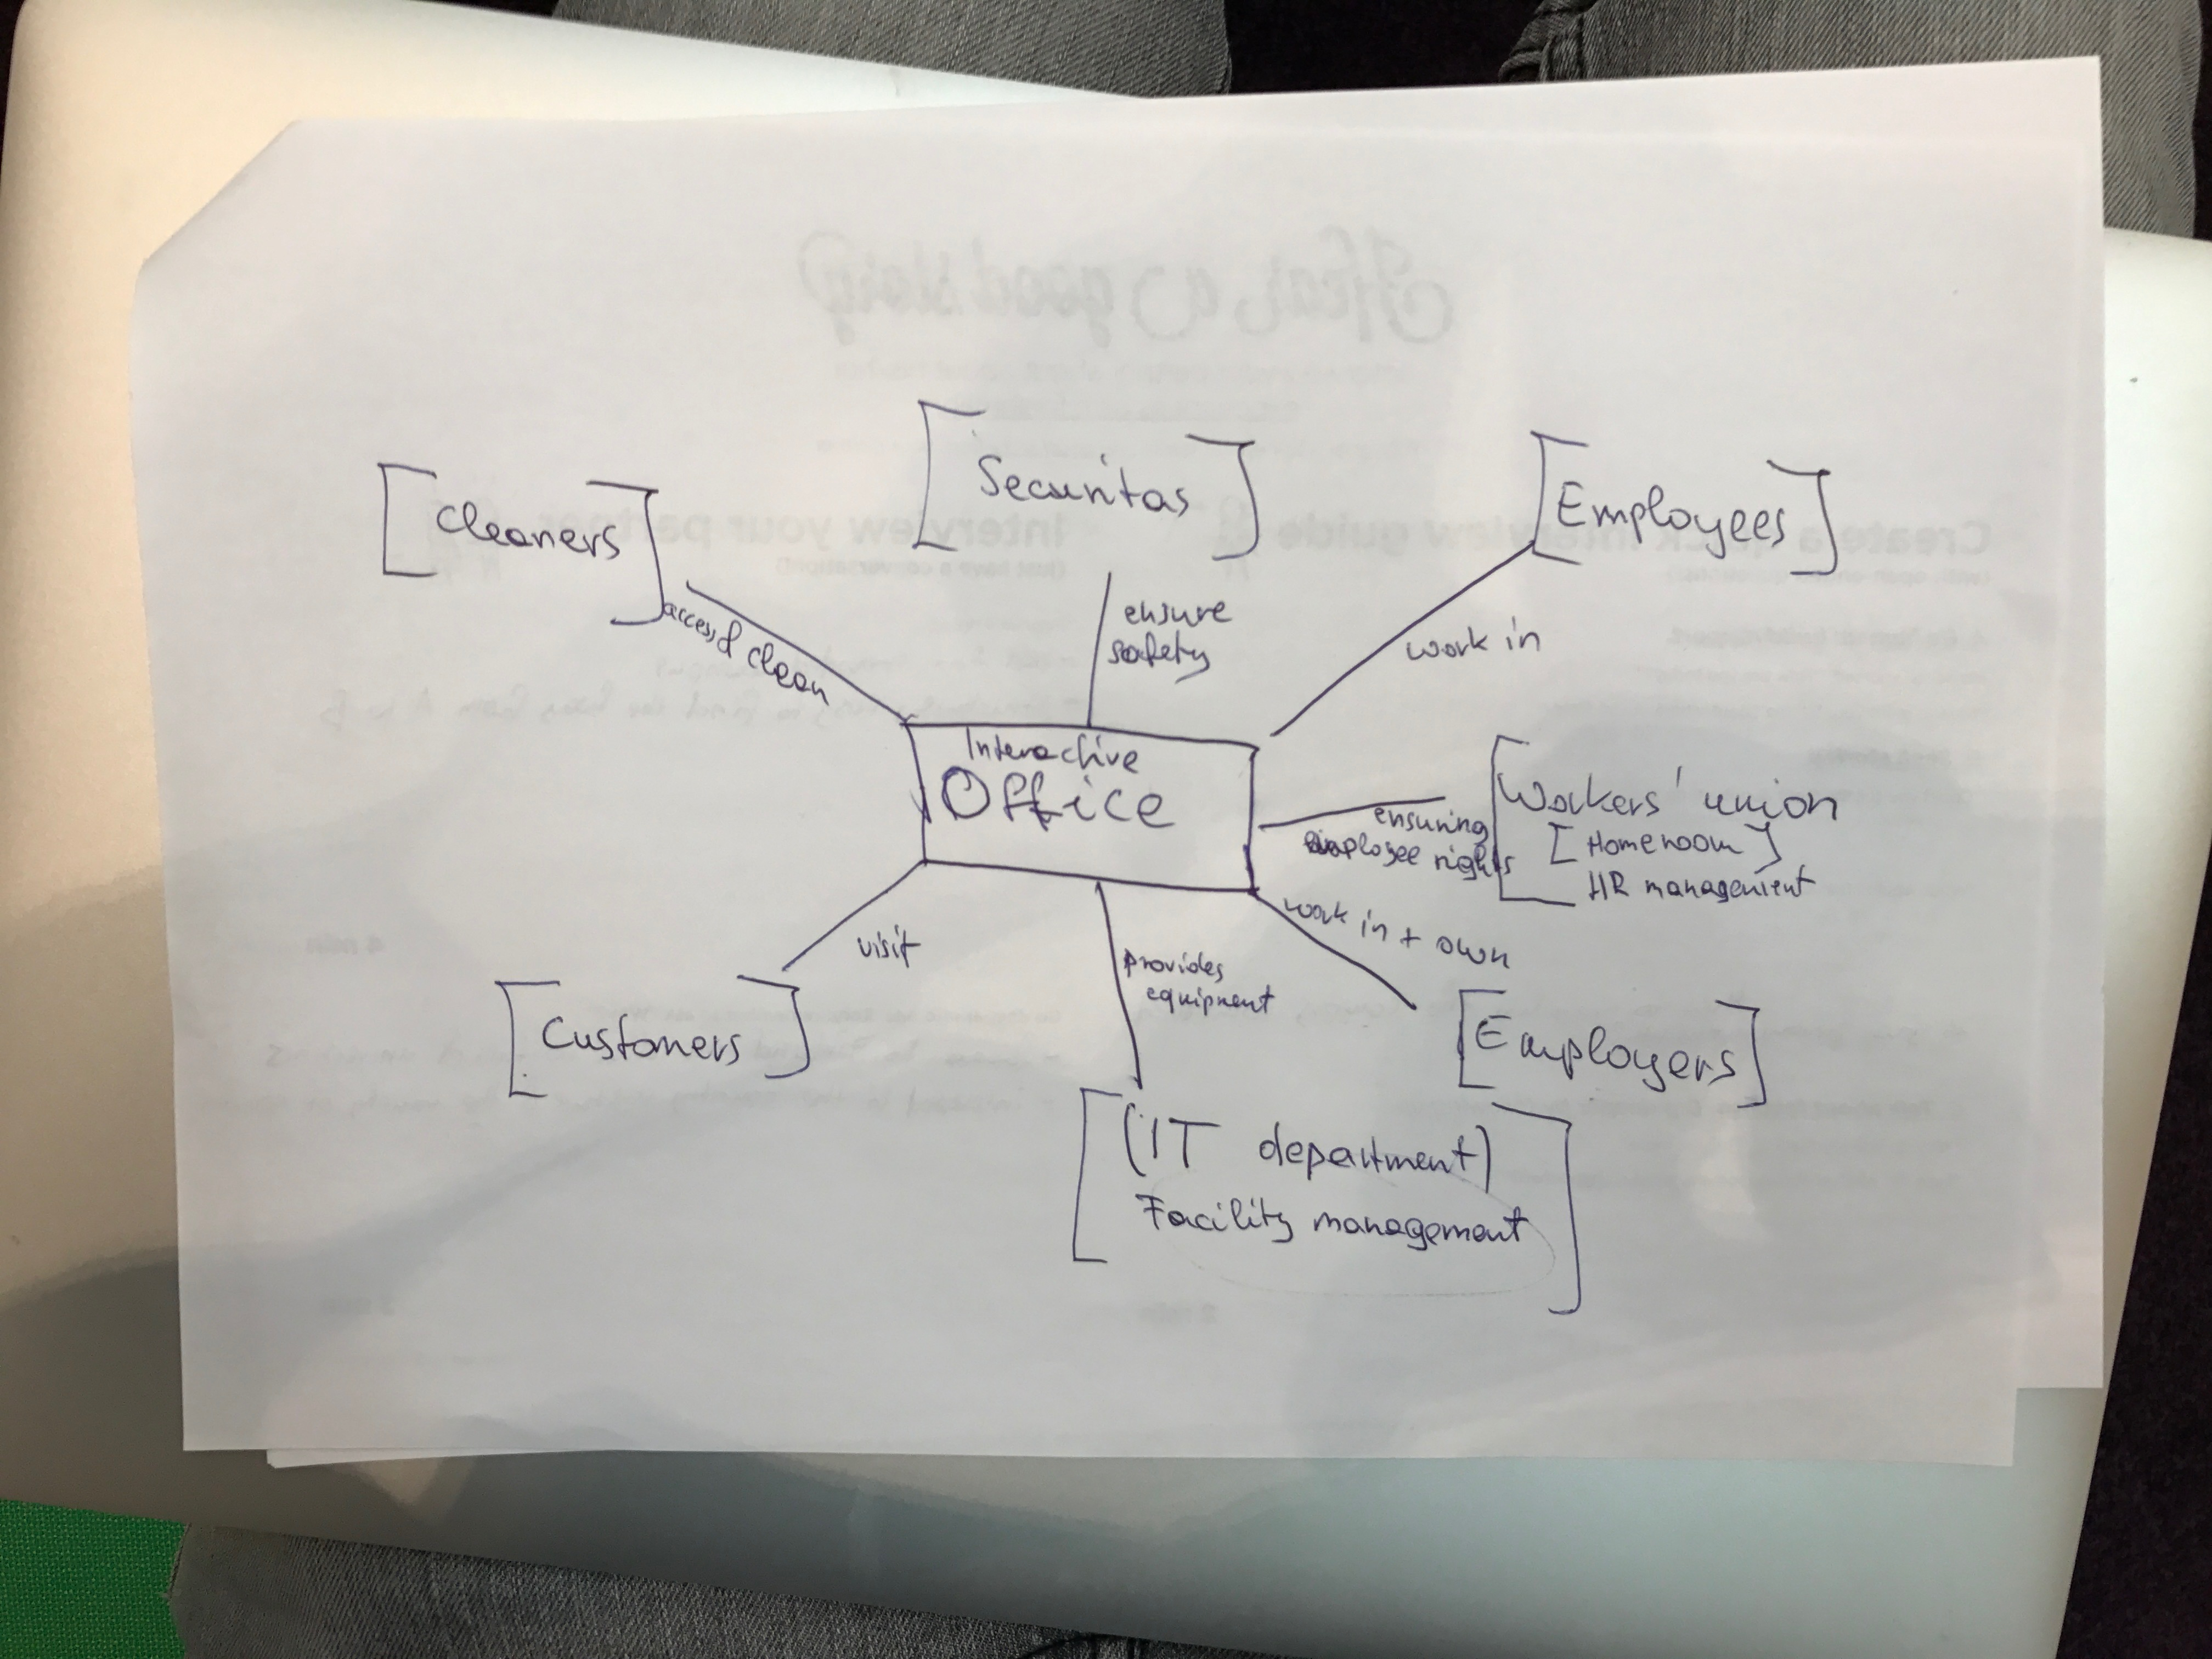
\includegraphics[width=0.9\textwidth]{images/stakeholdermap.jpg}
			\caption{The stakeholder map in an office environment.}
			\label{stakeholder_map}
		\end{center}
	\end{figure}

% what are the connections between the stakeholders? 

\subsection{Social Data Analysis}
Since the goal of our project is to solve an existing need, a social data analysis was conducted to 
identify potential areas of improvement. Multiple blogs and other internet sources were investigated 
and compared with each other to identify common patterns and areas of interest for the smart or 
interactive office. This section will outline the four key-areas that were identified in the social 
data analysis.

\paragraph{Efficiency}\label{sec:sda-efficiency}
Improving the efficiency of workers is one of the key drivers of change in workplace strategies 
according to \cite{hub13}. A smart or interactive office can help with this goal. Tools and software 
can help to reduce the time employees spend on tasks that are not directly related to profitable 
goals of the company.

Both \cite{iotagenda} and \cite{roomzilla9} describe that managing rooms is a tedious task. 
Roomzilla -- a software company selling room booking software -- estimates in \cite{roomzilla9} how 
much cost managing rooms without software can cause. The authors assume that office manager managing 
room bookings spends around 90 minutes per day to do so. Based on the average salary of an office 
manager in the US (\(20,65\text{USD}\)) the final estimate of this task is around \(681,45\text{USD}\) 
per month. The authors also mention some problems that can cause hidden costs: both late running 
meetings and overbooked rooms prevent employees from using their time to do actual work. 

The authors of this article instead describe how tracking room usage can lead to a better use of 
time. They propose a system that tracks room usage and makes the data available via Outlook or an 
appropriate alternative. This also helps employees to find a room when needed and therefore leads to 
less distractions and waste of time \cite{iotagenda}.

The tracked usage patterns can be utilized to save time and also to conserve energy. A smart or 
interactive office can turn on lights and devices in advance. In turn, the lights and devices can 
also be switched off when they are not needed anymore \cite{hbcommunications}.


\cite{hbcommunications} also outlines how AI and machine learning could be used to save employee 
time. They use the example of a smart call system with an automated menu that learns to direct calls 
to the correct department. This will reduce the time that is spent on redirecting callers and 
therefore improve the employees' efficiency. However, machine learning could also be used to suggest 
the best meetings times or predict when rooms are available.

Some other causes of wasted time in companies are technical problems in \cite{roomzilla3}. 
Especially in meetings these problems can take up some time. Sub-optimal setups, used (but not 
booked) rooms, and technical failures can cause delay of the meeting start and as such potentially 
lead to long-running meetings. The authors of \cite{roomzilla3} propose streamlined processes to 
make meetings more efficient. 

\paragraph{Collaboration}\label{sec:sda-collaboration}
Another key factor for innovation in the office outlined by \cite{hub13} is the hunt for and 
utilization of talented people. One major factor of keeping employees happy is to support different 
styles of work. This includes silent working areas to focus on projects, rooms to receive phone 
calls, but also areas where ``the atmosphere is conducive to innovation'' \cite{tieto}.

If these areas are provided, the employees must be able to freely move between these areas. One 
solution for this are non-fixed working desk, i.e. employees pick their working place when after 
they arrive in the office. \cite{occupiee}.  also outlines that flexible offices are needed as more 
employees work mobile and may rarely return to the office. In a flexible office environment with 
shared desks, the smart and interactive office must provide ways to find out where space is 
available and where colleagues are currently working \cite{tieto}.

Such technologies can be also be utilized to improve working together. If a project requires 
specialists, spontaneous meetings can be held by seeing who's currently available, where they are 
and what meeting room can be used \cite{tieto}. Similar results are mentioned \cite{hbcommunications} 
where the authors describe how streamlined communication and improved connectivity leads to better 
and faster collaboration between organization experts \footnote{\cite{hbcommunications} also 
mentions how automation of heating and lighting can lead to a more ``fun'' office improving the 
well-being of employees.}.

The importance of exciting workplaces for the creativity of employees is also mentioned in 
\cite{roomzilla3}. While typically it is assumed that such a playful environment may be detrimental 
to the productivity of employees, such environments can actually lead to a more creative and 
productive employees \cite{metroffice}. This in turn leads to better results and therefore a more 
successful business.



\paragraph{Comfort}\label{sec:sda-comfort}
Modern LEDs provide great ways to improve the worker's productivity by adapting intensity and the 
color spectrum. It has been shown in recent research that the color spectrum directly influences the 
activity and biorhythms of people  \cite{living-lab}. \cite{iotagenda} also highlights, how smart 
lighting can be used to create a more comfortable working environment.

Another important factor of well-being is acoustics. Most open area offices are too quiet and as 
such talks between colleagues and phone calls distract other people. However, too loud environments 
are also detrimental to work. Therefore the right balance as to be found \cite{living-lab}. 

Another possibility of the smart and interactive office is the automatic regulation of room 
temperature based on the time of day. Both \cite{iotagenda} and \cite{living-lab} outline the 
importance of temperature in the well-being of employees. People expect good thermal regulation in 
the office and it is also necessary to focus on work. But not everybody does feel temperature the 
same way. The living lab therefore developed and currently a ``climatic chair'' that helps each 
individual to regulate his or her working surrounding temperature \cite{living-lab}.


\paragraph{Safety}\label{sec:sda-safety}
Industrial workplaces like factories can be dangerous. While this is not directly related to a smart 
or interactive office, it is nonetheless an important factor in a smart workplace. \cite{sda-wired} 
lists a deadly accident which could possible have been prevented by utilizing modern technology.

In January 2012, one worker of the ArcelorMittal Burns Harbor steel-mill died while investigating 
noise in an oxygen furnace. The cause of death was a bursting pipe that released hot steam. The 
burst was caused by previously built-up pressure. A smart workplace could have prevented this 
accident by tracking pressure data in the pipe and warning workers to keep clear of the dangerous 
area.

Possible implementations of such a system could use apps, mobile devices, and wearables. In case of 
danger, acoustic and visual notifications could be send to the user. While such devices are widely 
available, \cite{sda-wired} mentions that software is lacking behind. The software of such systems 
must be intuitive to use. Also, the whole office and workplace has to be integrated: IT, machines, 
sensors, and finally the workers' devices. Since sensors produce a lot of data, \cite{sda-wired} 
also mentions that improved algorithms for streamed data analysis are needed.

\paragraph{Results}
The social data analysis verified, that a smart and interactive office can help to improve the 
efficiency of employees in various ways. One need that many of the papers outlined was the 
well-being of individuals because comfortable employees will produce better results.

Another important area was collaboration. This area can be improved by providing flexible working 
environments and better ways of communication. While some tools exist in this area, there is still 
way for improvement. 

Another final point which was identified is missing automation: much time is wasted by employees 
doing things manually that could be supported well by tools. Many of these tasks may be repetitive 
and also prevent the employee from doing ``actual work'' -- which in turn provides the chance to 
remove or simplify these automatable tasks.


\subsection{Observation}
To gain more understanding on the needs, an observation was carried out by the researchers. The reason for choosing this way of data collection is mainly triangulation, which provided us knowledge on the investigated domain from a different angle. On top of that, one of the team members works in an IT office environment in Helsinki, which allowed us to live with this possibility. For sake of confidentiality, the name of the firm and the exact details remain hidden in this report. 

The observation is carried out on a regular workday in the office when most of the employees are present. The room in which the observation is done is shared with four other colleagues. The observed environment is in between a corridor and another room in which other people are working. Therefore, there are multiple people actively working in the room, while occasionally others pass through. Accordingly, the environment is fairly noisy in general and there is some movement and interaction between employees. The room is equipped with rising desks and a whiteboard, that is used for work often by the employees. 

The observed insights and their short descriptions are, as follows:

\begin{enumerate}
	\item \textbf{Arrival to the office}: the first employees started to come around 9 AM and began to work in piece. As more and more people arrived to the office, the level of noise, interaction and movement increased naturally. Typically newcomers greeted their colleagues and initiated casual conversations with fellow coworkers (e.g. by asking how are you today, how was last afternoon, did you get stuck in the traffic as well?). However, some workers just entered the room with a coffee, sat down and began to work. 
	\item \textbf{Meetings}: around 10 AM, some colleagues left for a regular Daily Scrum meeting, which was hosted in another room. Throughout the working days, there are many prescheduled and recurring meetings, which are always hosted in one of the meeting rooms. Others left to their own private meetings/Skype calls during the day so that others are not disturbed and remain focused. In some cases however, people had ad-hoc face-to-face meetings or phone calls in the room which increased the level of noise and disturbance towards others.
	\item \textbf{Noise and interruption}: noise tended to be disturbing in some situations to employees. In most cases once somebody entered the room, he or she began to talk to one of their colleagues which dragged the attention of other workers in the zone. The disturbed employees either joined the conversation (which was either casual or work-related) and changed their attention from their computers to the person who just entered the room. This may or may not be a problem as these interruptions can be constructive to employee relationships or knowledge sharing in the company, but some may consider them as unnecessary interruptions. 	
	\item \textbf{Light in the room}: one interesting observation made during the day was pointed out by one of the employees in the office. Namely, the room has only one window and there is no natural light source coming in from the street. This fact is annoying for employees who work in this room for a long time as days are very short during the Finnish winter and there is not too much natural light whatsoever. For this reason, the company installed a device (similar to the one displayed on Figure \ref{artificial_sunlight}) that provides artificial sunlight that is turned on most of the day. 
	
	\begin{figure}[h] 
		\begin{center}
			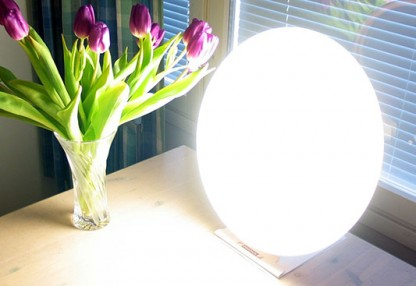
\includegraphics[width=0.9\textwidth]{images/artificial_sunlight.jpg}
			\caption{The office is equipped with a device that provides artificial light to the room with weak access to natural sunlight (the picture is only an illustration).}
			\label{artificial_sunlight}
		\end{center}
	\end{figure}
	\item \textbf{Interaction and breaks}: despite the morning chit-chat and the meetings, colleagues did not interact too much. Mostly, people were into their computers and their work, some even so much that seemingly they did not take any break despite lunch. 
	\pagebreak
	\item \textbf{Cleaning service}: at the end of the day, the cleaners arrived to the office. Their duties during workdays seemed to be limited to gather all glasses and cutlery from the desks of the employees and bring them to the common kitchen on the floor. Seemingly, the only cleaning lady had to make several rounds between the kitchen and the different rooms as the employees left many dishes all around the office. This seemed to be time consuming and probably would have been much faster if the items would be in the kitchen already. 
\end{enumerate}

\subsection{Interviews}


\section{Discussion}
\subsection{Research methods}
% what research methods are chosen

\subsection{Resources}
% what resources are utilized for carrying the project out? 

% what technologies, development principles are chosen and followed and why? 

%what do we build upon?

\subsection{Proposition}
% what do we propose? 

% what are the scenarios in which the solution can work? 

\subsection{Results and evaluation}

\section{Conclusions and future plans}

\pagebreak
\nocite{*}
\bibliographystyle{tktl}
\bibliography{references}


\lastpage
\appendices
\pagestyle{empty}
\singlespacing

\internalappendix{1}{Break habits \& collaboration during work - Interview questions}
Before asking the questions below to the interviewee, introduce your and the project?s background. Ask permission from the interviewee, if he/she has 10-15 minutes time to conduct the interview with you. Point out that the interviewee will remain anonymous. If you would like to record the session for further reference and analysis, make sure to ask permission.

\begin{enumerate}
\item Please introduce yourself shortly!
\item Tell me about your working field and environment! 
\item Do you think you take enough breaks during your work? 
\item Describe what do you do during your breaks! What do your breaks like? 
\item Do you interact with others during your breaks? 
\item Do you talk about work-related issues during your breaks? 
\item Do you know the professional skillset and hobbies of your colleagues well?
\item What is the standard way to in your organization to get to know the skillset of co-workers? 
\item Do you know whom to contact if you have work-related question? Are these people easy to reach? 
\item What do you do when you are stuck at work? 
\item What could be the reasons if collaboration between colleagues are not fluent/good? 
\end{enumerate}

\internalappendix{2}{Meeting minutes (2017.03.07. 14:00)}
Present members: 
\begin{enumerate}
\item Michael Morasch
\item Jan Lippert
\item Peter Ivanics
\end{enumerate}

Report: 
\begin{itemize}
\item Peter started writing the final report
\item Introduction paragraph and topic description is more or less done
\item Jan will summarize the social data analysis by next week which will be added to the report as soon as it is done
\end{itemize}

Interviews:
\begin{itemize}
\item Peter typed in the interview questions
\item Jan transcribed the pilot interviews and uploaded them to the Google Drive folder 
\item Peter will conduct an interview with one of his colleagues and a friend who is working by the next meeting
\item Michael will conduct interview with at least two people of his network by the next meeting
\item Jan will conduct one more interview
\item The new interview transcripts will be uploaded to the same Google Drive folder as above 
\end{itemize}

Responsibilities from this point onwards: 
\begin{itemize}
\item Michael: technical part, (backend) implementation
\item Jan: user evaluation, interviews, surveys
\item Peter: final report and project planning
\item Luca: ?
\item Who will do front-end related work, user interface design and prototyping? This remains a question for the next meeting.
\end{itemize}

Other issues: 
\begin{itemize}
\item The Gantt chart created by Peter was discussed
\item We agreed to finalize the needfinding and the careful analysis of the collected data and began prototyping by the Design Critique on 5th April 
\item Michael is in Finland until approximately 10th April - he will attend the design critique but cannot be on the demo day
\end{itemize}

Next meeting: \textbf{16th March, Tuesday, 14:15, 2nd floor of Exactum}

Topics: 
\begin{itemize}
\item Analysis of interview data
\item Clarification of responsibilities
\item Further planning of prototyping
\item Update on report statues, if there is time
\end{itemize}

Adjournment: we close the meeting at 14:33

\internalappendix{3}{Related Work}
Studies in real working environments are hard to do: the situation cannot be controlled and the 
study must impact the working people as less as possible. To conduct research, a controlled 
environment is needed. Researchers at the university of Kaiserslautern created the living lab to 
merge these requirements. The living lab is an open space office that was designed with the goal to 
conduct research in the area of Smart Offices \cite{living-lab}.


The living lab has researched different types of technologies. Examples include electrochromatic 
glass which can be turned dark on demand to prevent sunlight from shining trough or personlaized air 
flow optimization for workers. The living lab tests these technologies in simulations and real life 
situations. Another area of research is light and acoustic optimization. Good lighting and acoustics 
cannot be measured directly as most people only notice bad lighting or bad acoustics \cite{living-lab}.
\end{document}